\question[10] Consideren los cilindros de la Figura \ref{fig:20230319103650}:

\begin{figure}[H]
    \centering
    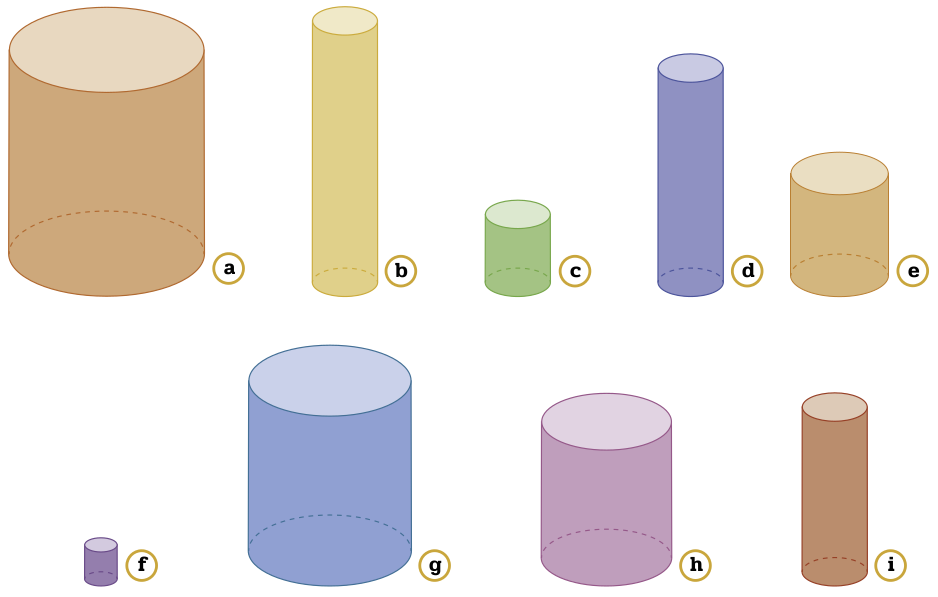
\includegraphics[width=.9\linewidth]{../images/20230319103650}
    \caption{}
    \label{fig:20230319103650}
\end{figure}

\begin{parts}
    \part Numera los cilindros en orden ascendente según su volumen.

    \begin{solutionbox}{1.5cm}
        $f$, $c$, $i$, $e$, $d$, $h$, $b$, $g$, $a$.
    \end{solutionbox}

    \part Si el volumen del cilindro $e$ es de 750 cm$^3$, estima qué cilindro tiene volumen de 1000 cm$^3$.

    \begin{solutionbox}{1.5cm}
        Se busca que el alumno seleccione los cilindros con una capacidad ligeramente mayor al $e$, tales como $d$, $h$ o $i$.
    \end{solutionbox}

    \part Estima cuál es el volumen del cilindro más grande. Explica.

    \begin{solutionbox}{1.5cm}
        El cilindro $a$, se estima que su volumen es 4 veces el de $e$, es decir, de 3000 cm$^3$.
    \end{solutionbox}

    \part Estima qué volumen tiene el cilindro más chico.

    \begin{solutionbox}{1.5cm}
        Es el cilindro $f$, se estima que su volumen es la décima parte de $e$, es decir,
        de 75 cm$^3$.
    \end{solutionbox}
\end{parts}